\section{Museum Lighting}

\bigskip

\begin{quote}
`Museums and art galleries collect, preserve, and display natural artifacts and/or examples of human achievement and analyze their impact on the world and the universe around us. Effective exhibit lighting must balance exhibition and conservation needs and enrich the museum experience.'
\end{quote}

\begin{flushright}IES RP-30-96 Museum and Art Gallery Lighting: \\A Recommended Practice \citep{ies_ies_1996}\end{flushright}

\bigskip

Lighting in museums is required to satisfy multiple criteria; perhaps the least contestable requirement being that the lighting illuminate objects such that they are suitably visible to museum visitors. Also of utmost importance in most museum settings is that the lighting does not have an unreasonably damaging effect upon the objects or environment, be this through direct photodegradation or as a result of heat transfer. Further to these requirements, an increased or optimal visual quality is generally desirable, although what this represents or how to achieve it is generally ambiguous.

In sweeping terms, all electromagnetic radiation (visible and non-visible) damages objects, and more radiation damages objects proportionally moreso. Thus the question becomes: \emph{how little light can we use to illuminate objects such that they're visible to the extent required?} The inverse form, sometimes used on the assumption that more light always represents an increase in observer satisfaction/pleasure is: \emph{`how much light can we use so that only $x$ damage occurs over $y$ time'}. 

Industry guidance documents provide advice on how to manage lighting to best address the above requirements and many other additional specific requirements through the recommendation of procedure and provision of target figures for quantitative variables. \Gls{UV} radiation, being of no visual benefit but having potential to harm, is now excluded from gallery spaces as an industry standard.

\subsection{Damage functions} \label{sec:DamageIndex}

In heritage science `damage functions' are ``functions of unacceptable change, dependent on agents of change''\citep{strlic_damage_2013}. The goal of damage functions in heritage lighting engineering is to give a quantitative means by which to predict the amount of damage caused to a prototypical object by a given light source, and to assist in limiting such damage. They generally follow the logic that radiation of lower wavelength is likely to cause more damage to objects.

\citet{harrison_report_1953} is generally acknowledged as the first to suggest such a function, but he himself acknowledges that it had ``long been established that the shorter the wavelength (visible yellow, green, blue, violet and invisible UV being progressively shorter) the more photochemically potent will be such radiant energy, provided such energy is actually absorbed''. \citet[p.9]{harrison_report_1953} defined the `radiation hazard associated with a light source' as:

\begin{equation}
    \sum_{0}^{\infty} \mathrm{H}_{\lambda} \mathrm{D}_{\lambda} \Delta \lambda / \sum_{0}^{\infty} \mathrm{H}_{\lambda} \overline{\mathrm{y}}_{\lambda} \Delta \lambda
    \label{eq:Harrison}
\end{equation}

where $\mathrm{H}_{\lambda}$ is the spectral irradiance, $\mathrm{D}_{\lambda}$ is the `Relative Damage Factor' (which is extrapolated from the data collected shortly prior to Harrison's own report by the National Bureau of Standards \citep{noauthor_preservation_1951}, and shown in Figure \ref{fig:Harrison}), and $\overline{\mathrm{y}}_{\lambda}$ is the CIE 1924 photopic $V_{\lambda}$ luminosity function. The resulting value would describe the amount of damage expected from a light source, normalised by its luminance.

\begin{figure}[htbp]
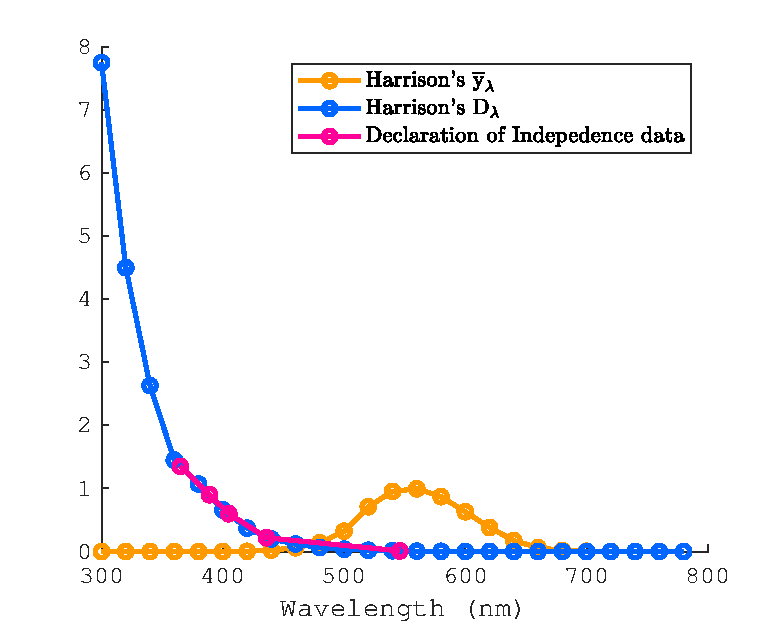
\includegraphics[max width=\textwidth]{figs/LitRev/HarrisonInd.pdf}
\caption{Harrison's \citep{harrison_report_1953} damage function ($\mathrm{D}_{\lambda}$), and luminous efficacy ($\overline{\mathrm{y}}_{\lambda}$), alongside the Declaration of Independence data \citep{noauthor_preservation_1951} from which it was extrapolated (re-normalised to match scale).}
\label{fig:Harrison}
\end{figure}

\begin{figure}[htbp]
%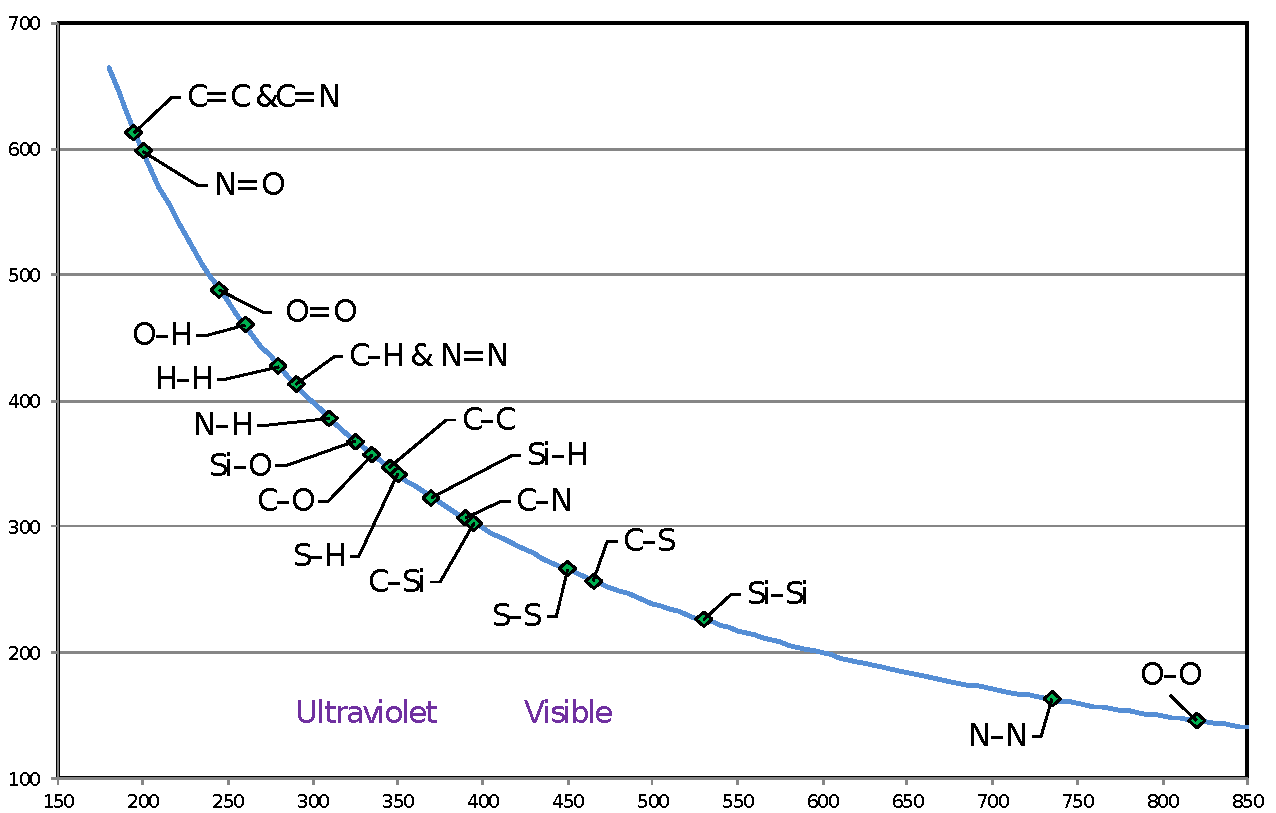
\includegraphics[max width=\textwidth]{figs/LitRev/Saunders.pdf}
\caption{Graph courtesy of David Saunders, presented at the Museum Lighting Symposium \& Workshops \citep[p.61]{pokorska_book_2017} showing the relationship between wavelength and the bonds which can be broken in various molecules, with `Wavelength (nm)' on the abscissa and `Bond energy (kJ/mol)' on the ordinate.}
\label{fig:Saunders}
\end{figure}

There has been extended scepticism about the utility of damage functions in general, with the argument being that no one damage function could represent the vast range and complexities of real materials. \citet[p. 178]{thomson_museum_1978} wrote that ``for more fugitive materials \dots the figure for visible radiation would be higher. On the other hand \dots the fastest dyes are probably affected only by UV. Thus it can be seen that no single figure can be given for damage versus wavelength''.

Criticism was aimed at this specific damage function due to it's derivation from such a small and minimally representative dataset - Harrison's data was `extended' from the 5 datapoints measured by the National Bureau of Standards \citep{noauthor_preservation_1951} in their investigations of how to best care for the Declaration of Independence\footnote{It is a curiosity that these minimal figures would not in fact have been much use to those planning the care for the declaration, since in the report it is noted that ``The deterioration of animal parchment is not as rapid as that of the low-grade paper for which the damage factors were determined''\citep{noauthor_preservation_1951}, and the Declaration of Independence is written on animal parchment.}, and was derived from the study of `low-grade paper', which cannot to said to represent the average museum item\footnote{Though \emph{no} material truly can!}.

CIE 157:2004 \citep{cie_cie_2004} notes that whilst Harrison's proposal failed to gain acceptance as the procedure for comparing the damage potential of different types of light sources, it did convince people of the ills of \gls{UV}, with the result that daylight was subsequently eliminated from many galleries.

Following \citet{cuttle_lighting_1988}, who noted that Harrison's damage function could be well fit by an inverted logarithmic function, with parameters controlling the slope and normalisation point of the function, CIE 157:2004 provided the following equation:

\begin{equation}
    s(\lambda)_{\mathrm{dm,rel}}=\exp [-b(\lambda-n)]
\end{equation}

where differing values of $b$ for 5 categories of item are provided (Table \ref{tab:b}), $n$ is the normalisation value (CIE 157:2004 uses a value of 300), and the $s(\lambda)_{\mathrm{dm,rel}}$ function is the estimated action spectrum for each category. $s(\lambda)_{\mathrm{dm,rel}}$ would be substituted into Equation \ref{eq:Harrison} for $\mathrm{D}_{\lambda}$. CIE 157:2004 also provides values of $H_{s,dm}$ which indicate the susceptibility of each group of materials to damage (where damage is considered as colour change%in $\Delta E_{\mathrm{ab}}^{\ast}$
).

\begin{table}[htbp]
\centering
\begin{tabular}{|c|l|l|l|}
\hline
Group & Samples & $H_{s,dm}$ (W h/m$^{2}$) & $b$ \\ \hline
a & Low-grade paper & 5 & 0.038 \\ \hline
b & Rag paper & 1200 & 0.0125 \\ \hline
c & Oil paints on canvas & 850 & 0.0115 \\ \hline
d & Textiles & 290 & 0.0100 \\ \hline
e & Water colours on rag paper & 175 & 0.0115 \\ \hline
\end{tabular}
\caption{Table reproduced from CIE 157:2004 \citep{cie_cie_2004}, showing the values for $H_{s,dm}$ and $b$ for various categories. Note: the source for this data is not particularly clear; it is listed as `The Berlin researchers', which is assumed to follow the references: \citet{krochmann_beleuchtung_1988,cie_cie_1991,hilbert_zur_1991}, none of which I have been able to access.}
\label{tab:b}
\end{table}



\noindent
X extended Harrison's data to other types of object \dots

\noindent
Luminance is crappy.

% disregarded
% altogether although the D{~,~ function shows wavelength
% weighting varying over a 10: 1 range in this region.
% The argument, then, is not whether we have a D(h) function
% which is correct, but whether we can improve usefully upon
% the likely reliability of the present system.

\noindent
Radiation must be absorbed \dots \citet{durmus_optimising_2017,durmus_colour_2015,durmus_optimising_2015,durmus_object_2017}. \citet{saunders_wavelength-dependent_1994}, \citet{villmann_wavelength_2018}

With modern computation, and access to datasets, it becomes relatively easy to calculate a value of \Gls{DI} (as per Equation \ref{eq:Harrison}), but further normalised such that Illuminant A has a reference value of 1). Figure \ref{fig:Houser} shows the results for such computations for 401 illuminants and light sources\footnote{The code to reproduce this is available from: \url{https://github.com/da5nsy/DamageIndex}}.

\begin{figure}[htbp]
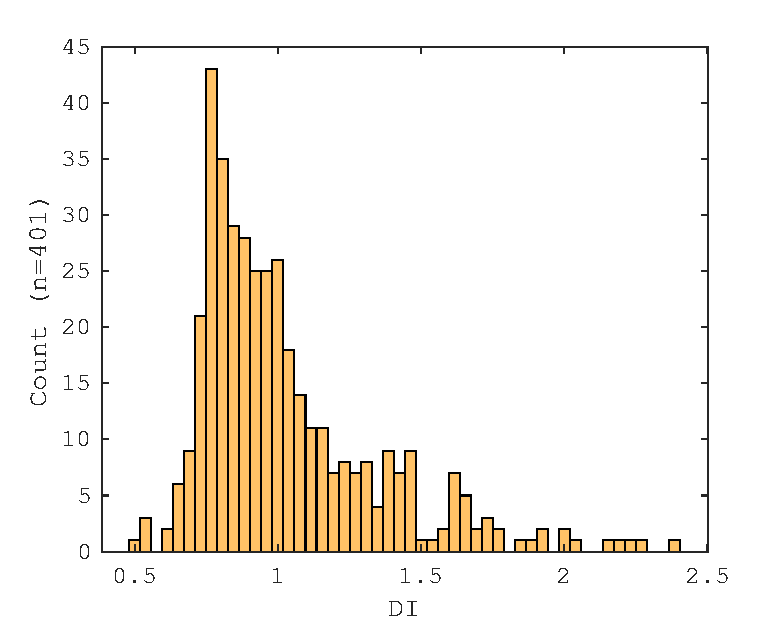
\includegraphics[max width=\textwidth]{figs/LitRev/DI.pdf}
\caption{The values of $DI$ }
\label{fig:Houser}
\end{figure}

\subsection{Interviews with Museum Professionals} \label{sec:Interviews}

\textit{The following work has been published as \textbf{`How is museum lighting selected? An insight into current practice in UK museums'} \citep{garside_how_2017}. An overview is presented here, focusing on the elements relevant to the rest of the thesis, rather than as an independent chapter.}

\medskip

In order to gain an understanding of how museum professionals currently specify lighting, interviews were conducted with 12 museum professionals representing 10 UK based museums, galleries or historic property management groups, in spring of 2016. A small number of these professionals represented UK-wide groups, but the majority represented London based institutions.

The interviews were semi-structured around a set of questions composed by the author and their academic supervisors (reproduced in \citet{garside_how_2017}). The choice to conduct these interviews in a semi-structured format as opposed to a fully-structured one was based on the desire to allow unanticipated topics to enter the conversation, so as to limit the potential for important subjects to be neglected due to naivety of foresight. The conversational format of the interviews meant that the resulting data was qualitative rather than quantitative, which to an extent hinders comparison, but it was decided that the variety of job roles and institutional sizes, and the small sample size, already made quantitative comparison of limited meaningfulness for this investigation.

The interviewees were contacted through introductions from supervisors, personal connections, or cold emails. Almost all held conservation based roles (the exception being an `exhibitions manager') and noted that their principal responsibility regards lighting was controlling the safety of lighting regards its ability to cause damage to the objects held and displayed by their respective institutions. This generally involved monitoring and analysis of existing lighting systems and natural illumination, creating general guidance documents for the specification of lighting in their specific institutions and for loan items, and providing guidance and recommendations for the fitting out of new galleries or gallery refits. Few considered themselves directly responsible for the appearance of museum objects, considering this to be a creative decision outside of their remits. Future work considering the perspective of others involved in museum lighting, such as representatives from external lighting design companies, is required.

Whilst a small number considered themselves active in the area of lighting research, all interviewees were responsible for more conservation considerations aside from lighting, limiting the practicable level of specialisation. Many considered communication and dissemination a key part of their role, often noting they often found themselves in the position of needing to educate other teams within their institution on subjects including lighting. 

\begin{quote}
``This is not my science, my job is pulling it out and presenting it to others.''
\end{quote}

Asked what each considered to be `good lighting', responses included `safe', `invisible' (you don't notice it), and `lighting which is appropriate for your objects and your exhibition' (noting the variability of requirements dependent on the particular object(s) being presented). Asked to present a list or range of priorities, many focused on the safety requirements of lighting. The principal safety concern for lighting was that it fell below specific illuminance criteria, dependent on the assumed sensitivity category of the object in question. The specific target values were generally those provided by \citet{thomson_museum_1986} of 50lx for sensitive items and 200lx for less sensitive items (which are based on the visual preference work of \citet{loe_preferred_1982}).

Considering a scale of other priorities, following the requirement for appropriate lux levels, considerations included: limiting/excluding \gls{UV}, obtaining an acceptable \gls{CRI} value, and time and capital costs associating with fitting and maintenance. Energy efficiency was also a driver, but this did not seem to be a factor within technology category, rather it was noted that many institutions are switching to \gls{LED} because of increased efficiency, but that the difference in efficiency between one \gls{LED} type and another was negligible compared to the saving in contrast to lighting technology which \gls{LED} was replacing, which was often tungsten.

The range of roles played in the procurement of lighting varied amongst those interviewed. Whilst some created guidance documents which would then be passed on to estates teams and exhibition designers or lighting designers specifically, others had a much more hands-on role, testing specific lighting before installation or making recommendations on a case-by-case basis. It was noted that whilst relamping and retrofitting was generally handled by `in house' teams, where new galleries or large temporary exhibitions were created it was common for an external lighting design company to be contracted to perform the work. When asked whether recommendations were normally followed, the general reply was that recommendations for lux exposure and UV content were almost always followed, but other recommendations (such as for \gls{CRI} or \gls{CCT}) were more loosely interpreted. In many cases recommendations for \gls{CCT} were not made.

When asked about the tools used to make such recommendations and choices, responses included references to guidelines and reference sources (most often \citet{thomson_museum_1986}, though also \citet{druzik_guidelines_2012} and \citet{british_standards_institution_pas_2012}), references to specific units such as `lux' used in tandem with recommendations from guidelines such as above, indices such as the \gls{CIE} general colour rendering index R$_a$ (referred ubiquitously to as `\gls{CRI}' by interviewees) and notes of specific conferences which were attended in order to stay up to date with the research on the subject. There was a general feeling that the current climate was one of swift technological change in lighting, which created an increased difficulty in staying up to date with developments. It was noted that attending conferences and industry workshops were very beneficial in assisting professionals to stay up to date. 

\begin{quote}
`   Things are moving so quickly that to rely on books which have taken two years to produce [does not suffice, because] things have moved on. Books (plus journals) used to be the main reference. Now things are moving at such a rapid pace.''
\end{quote}

A range of techniques were used to qualify whether specific lighting was `safe' or not. The most common practical technique was spot metering of lux values incident on specific objects, and selective dimming to drop incident lighting to the desired lux level in response to this. Some larger institutions with access to microfading equipment were able to use this in the determination of sensitivity of specific objects. One interviewee provided details of a spectral power distribution based method for considering the safety specifically of phosphor based \gls{LED} illumination, whereby the height of the blue peak was compared to the height of the peak of the broader peak above 500nm, and if the former was more than three times the height of the latter, that lighting was singled out as potentially not safe. Other interviewees had heard of this criteria, and some used it as a rough guide, but one remarked that it was `fairly arbitrary'. One of the most succinct and perhaps astute responses was ``what is `safe'?''. One interviewee referred to the website of \citet{padfield_relative_2012} where considerations for the `RE\%' (`relative spectral sensitivity normalised exposure values'), using the damage functions described by \citet{s._aydinli_deterioration_1990} are used.

The interviewees generally did not consider characteristics of the displayed objects such as geometry of illumination, broadly considering this to be the remit of a lighting designer or exhibition designer rather than a conservator.

One of the most interesting, and perhaps surprising findings was the ubiquity of visual testing of lighting, generally performed prior to any large installation. For relamping, manufacturer supplied attribute values were generally relied upon as this required less time/effort and was cheaper. The most common procedure for new installations seemed to be for an informal and minimal visual test to occur before widespread installation. In a single case however, visual testing was actively avoided (on the basis that visual testing could not deliver meaningful insights where the aim was accurate rendering as opposed to visually pleasing rendering) and in another case large scale visual testing was performed, including many different types/brands of lamp and a large number of museum staff, and a final decision was made almost entirely on the results of this testing.

\Glspl{LED} are now used, at least in part, in all the institutions involved in this survey. In several they are the primary lighting technology but in a small number they are used sparingly, only in applications such as the lighting of text information panels. In one they are used in a particularly minimal fashion, although this was attributed to the fact that the museum is moving location in the near future and thus capital investments in building infrastructure were being avoided for the present time. There was no one specific brand or type which seemed to be ubiquitous across institutions, rather each institution appeared to have relationships with different manufacturers and suppliers.

Most interviewees were aware of warnings which had been issued and well publicised in the mainstream press \citep{lewis_smith_will_2013} regards the potential of \gls{LED} sources to be especially degrading for specific objects. Interviewees saw these warnings as controversial and likely unwarranted, and were confident that research had been conducted which cleared \Glspl{LED} of causing an unacceptable level of damage in comparison with alternative technologies. When asked how they might assess a light source for safety, most replied that safety was assessed solely through use of an illuminance meter and lux targets, not through analysis of the \gls{SPD} or any other lighting attribute. Those who did critically assess the \gls{SPD} generally used no specific tools to do so, focusing attention on the wavelength of the spectral emission peak.

\begin{quote}
``We never normally adjust the lighting type for a given artwork, we adjust the intensity''
\end{quote}

\begin{quote}
``For all lighting we measure the \gls{SPD}, and check it is reasonable''
\end{quote}

They key driver behind the adoption of \Glspl{LED} appears to be energy efficiency increases and energy use reductions, as required by institution-wide directives, or as part of applications for planning permission. Secondary to this consideration, benefits noted include: decreased maintenance costs from extended lifetime of products, and a lack of availability of traditional bulbs, sometimes due to specific legislation which has in effect phased out some traditional technologies. One element holding back some interviewees from further investment was a residual feeling that this new technology was not yet fully proven. Many pointed out that the claims made regards extended lifetime of \Glspl{LED} were yet to be proven in real world environments due to the relatively new nature of the technology. Some also noted the high costs associated with having to change the underlying lighting infrastructure, where retrofitting wasn't possible or appropriate. A final note on this section - some interviewees were unsure about the ability of \Glspl{LED} to remain colour stable over the long expected lifetime of the products.

Interviewees reported that visitors had not generally responded to any changes in lighting technology, and this was taken to mean that any switch to \gls{LED} had not been negatively received. It was inconclusive whether or not the technology was positively received however. This could be a meaningful avenue for future work. In terms of the professionals own opinions of \gls{LED} lighting, all seemed favourable, though it was unclear how much of this effect was caused by extraneous or related effects such as a placebo effect due to the excitement of new technology, or different chromaticities or brightnesses of replacement technologies.  

\begin{quote}
``I like what I've seen. The galleries where we have just \gls{LED} spots, I feel happier. I went to [another institution, with abundant \gls{LED} lighting], I really like the galleries where they had \gls{LED} lighting, and it was more of a gut feeling rather than something which I could put my finger on, but actually, it felt cleaner to me.''
\end{quote}

Whilst all interviewees were interested in the idea of making objects appear brighter whilst reducing the level of damage caused, the point was made that whilst spectral tuning might benefit a prototypical object, it will not necessarily benefit real objects in real environments. It was also noted that the use of lux in making decisions was particularly problematic here, where varying the location of a blue peak could easily increase the level of damage but reduce the lux value.
Most interviewees had a basic understanding of colour temperature, and a limited understanding of chromatic adaptation. The colour temperature of lighting was generally not seen as a conservation issue (though there were exceptions to this), and rather as a creative consideration. One interviewee noted that it was manipulated to great effect by external lighting designers in order to create specific effects or atmosphere.

The justification for \gls{CCT} specification values generally appears to stem from two routes. Firstly, from guidance documents such as those provided by The Getty and the Canadian Conservation Institute \citep{druzik_guidelines_2012}, and secondly from a desire to match existing lighting, either daylight or more commonly tungsten (at around 3000K). It was rarely considered as a means to control damage, or as a way to enhance visual appearance, by those interviewed. One interviewee referred to the work of \citet{kruithof_tubular_1941} and \citet{scuello_museum_2004,scuello_museum_2004-1} as justification for choosing low \gls{CCT} illumination similar to tungsten. No specific issues relating to colour temperature were raised by interviewees.

The interviewees were very interested in the subject of accurate representation, and almost all seemed to regard accurate object representation as a key priority. The figures for R$_a$ quoted in internal documents at each institution were either 80, 85 or 90, as a minimum figure. In one institution, an R$_w$ value was calculated for each proposed light source (the R value of the test colour sample with the colour shift of greatest magnitude, aka `worst') and a cut-off of 80 imposed. However, most interviewees seemed unsure of the practical relevance of R$_a$, with many considering it a rough guideline which would be considered secondarily to a visual inspection of lighting.

Those who were particularly interested in the subject gave the impression that whilst the subject was considered philosophically in great detail, the tool which was actually used to analyse the colour rendering of a light source was still generally just R$_a$. A few interviewees were aware of TM-30-15 \citep{color_metric_task_group_of_the_ies_ies_2015}, and whilst it was respected, it was questioned whether it represented a real improvement over R$_a$.
On the subject of lighting philosophy, the opinions encountered generally aligned with the mechanics of R$_a$. That is to say; given a choice between illuminating an object such that it was beautified, visually restored (to a previous condition) or simply presented as it would appear under daylight/tungsten illumination, most opted for the final option. Whilst there was clear interest in the other options, and other creative ways in which to consider colour rendering, it was generally believed that the role of the museum should be to represent objects in an un-biased manner, and thus a fidelity index was an appropriate tool for discussing a light source's colour rendering properties. In the case where specialist lighting was used to special effect, the opinion was noted that \textit{`you have to be very clear about what you are doing and why'} in order to maintain the reputation of the museum as an arena for honest and unbiased representation.

Generally, the interviewees believed that visitor requirements were being met (although there is often difficulty in defining exactly what visitor requirements actually are) and no specific tool or technology was proposed that would provide a clear benefit. Several interviewees mentioned that a way to improve the accessibility of colour rendering indices (in terms of the ease with which they could be understood and applied) would be appreciated.

No interviewees knew of recent surveys similar to the present one.

\subsection{Visitor Requirements of Museum Lighting}

The visitor requirements of museum lighting are varied and complex. The examination and definition of these requirements has been the subject of a small number of studies, principally by \citet{kesner_museum_1993-1} in the USA in the early nineteen-nineties \citep{kesner_museum_1993,kesner_exhibition_1992,kesner_current_1991,kesner_analysis_1997}. These studies were based on survey based self-reporting, and concluded that colour accuracy was the highest requirement and that `richness' of colour was the lowest priority\footnote{A cautious interpretation of these results is advised, considering that there were high average scores for each category}.

\begin{quote}
Artifact appearance, particularly clarity of artefact form and accuracy of artifact color, is the most important visitor need. Although visual impression, specifically acceptable gallery brightness and rich artefact color, is least important among the factors, it too rated highly important \citep{kesner_museum_1993-1}.
\end{quote}

Further studies, spurred by recent adoption of \gls{LED} technology have been completed, although with very limited and questionably scientific basis at the Field Museum \citep{myer_demonstration_2010}.

Additionally work has been completed which describes the results of a written survey of museum professionals on the subject of lighting specification, focusing on SSL (effectively \gls{LED}) adoption, and their justification for specifying specific lighting \citep{perrin_ssl_2014}. 979 people who had requested access to the guidelines document produced by some of the same authors \citep{druzik_guidelines_2012} were emailed with a request for participation. 46 (4.7\%) responded with a completed survey. Of those, 30\% are described as `international' which considering the base of the authors is in the USA we can assume as meaning `not based in the USA'. The survey was prepared as part of the USA government's GATEWAY program, and can be considered as a follow-up to work on recommendations for specification \citep{druzik_guidelines_2012}. 

\noindent
The headline results are as follows:
\begin{itemize}
    \item When the `success' of new \gls{LED} based lighting schemes was evaluated the public reaction was either neutral or positive in all cases \footnote{There appears to be an issue with the data for this question however, with the `no response' garnering 48\% of the responses and `favorable response' garnering 55\%\dots}
    \item The distribution of staff response was broadly similar: `no response'-17\%, `negative response'-3\%, `favorable response'-80\%.
    \item The results of two priority ranking questions\footnote{`Rank the following lighting goals' and `Please rank the following factors in your selection of lamps'} are broadly similar:
    \begin{itemize}
        \item First question: The first priority is identified as `limiting damage' with other priorities broadly equal.
        \item Second question: Joint first priorities are identified as `colour and spectral power distribution' and `damage potential' with others broadly similar (though dimming, input power and warranty lagging behind others)
    \end{itemize}
    \item 91\% of respondents reported using `\gls{CRI}' which is assumed to refer to \gls{CIE} R$_a$. 6\% state that they refer to other Ri values, and 20\% report using CQS (Color Quality Scale \citep{ohno_rationale_2010,davis_color_2010}).
    \item 60\% of respondents report that they consider \gls{CCT}.
\end{itemize} 

\subsection{Museum Lighting Specification Guidance Documents}

Following the interviews with the museum professionals, the five most referred-to museum lighting guidance documents were reviewed, and a summary is presented here.

\noindent
The guidelines chosen for review were:
\begin{itemize}
\item The Museum Environment \citep{thomson_museum_1986}
\item \gls{CIE} 157:2004 Control of Damage to Museum Objects by Optical Radiation \citep{cie_cie_2004}
\item Guidelines for Selecting Solid-State Lighting for Museums \citep{druzik_guidelines_2012}
\item SLL LG8: Lighting for museums and art galleries \citep{cibse_lighting_2015}
\item IES RP-30-96 Museum and Art Gallery Lighting: A Recommended Practice \citep{ies_ies_1996}\footnote{This has since been usurped by \citet{illuminating_engineering_society_ies_2017}.}.
\end{itemize}

\noindent
In summary:
\begin{itemize}
\item Recommended values were provided for:
\begin{itemize}
\item \emph{Lux}: various, dependent on sensitivity, generally based on figures from the study of visual preference by \citet{loe_preferred_1982}.
\item \emph{R$_a$}: various, most frequently \textgreater 80, with no experimental basis referenced.
\item \emph{\gls{CCT}}: various, based implicitly on \citet{kruithof_tubular_1941} or on such ideas found empirically.
\end{itemize}
\item Most also suggested visual inspection as a valid means of assessment.
\item There was often blurring between recommendations concerned with visual appearance and those concerned with conservation. 
\end{itemize}

\subsection{CCT in museums}

\acrfull{CCT} describes the chromaticity of a light source on a one dimensional axis roughly from blue to yellow, based on the apparent chromaticity of a black body radiator at differing temperatures. It is often described as an important variable in museum lighting but definite recommendations, in the rare cases that they are given, are generally based on very general rules that predict that damage potential will be decreased if \gls{CCT} is minimised \citep{cie_cie_2004}, nostalgia for the appearance of tungsten lighting or questionable research on human preference \citep{kruithof_tubular_1941,fotios_revised_2017}. Whilst some research appears to have found optimal \glspl{CCT} for viewing artwork \citep{nascimento_best_2014,pinto_correlated_2008,scuello_museum_2004,scuello_museum_2004-1, liu_cultural_2013} results often have large inter-observer variability, context dependency and it is not uncommon for the headline findings of separate studies to be in contradiction. 

Specifications often refer implicitly or explicitly to the findings of \citet{kruithof_tubular_1941}, who found that at lower levels of illumination, lower \glspl{CCT} were preferred, and that at higher levels of illumination higher \glspl{CCT} were preferred. Whilst this general trend seems to have anecdotal support, it is possible that there may be lighting-technology-based confounds, and recently researchers \citep{vienot_kruithofs_2009} (including a meta-study of multiple other examinations \citep{fotios_revised_2017}) found there to be no provable correlation between preference and colour temperature.

The \gls{CIE} however, published a report showing the varying the \gls{CCT} of museum lighting could have a clear impact on the potential damage undergone by museum objects \citep{cie_cie_2004}. 

\begin{figure}[hbtp]
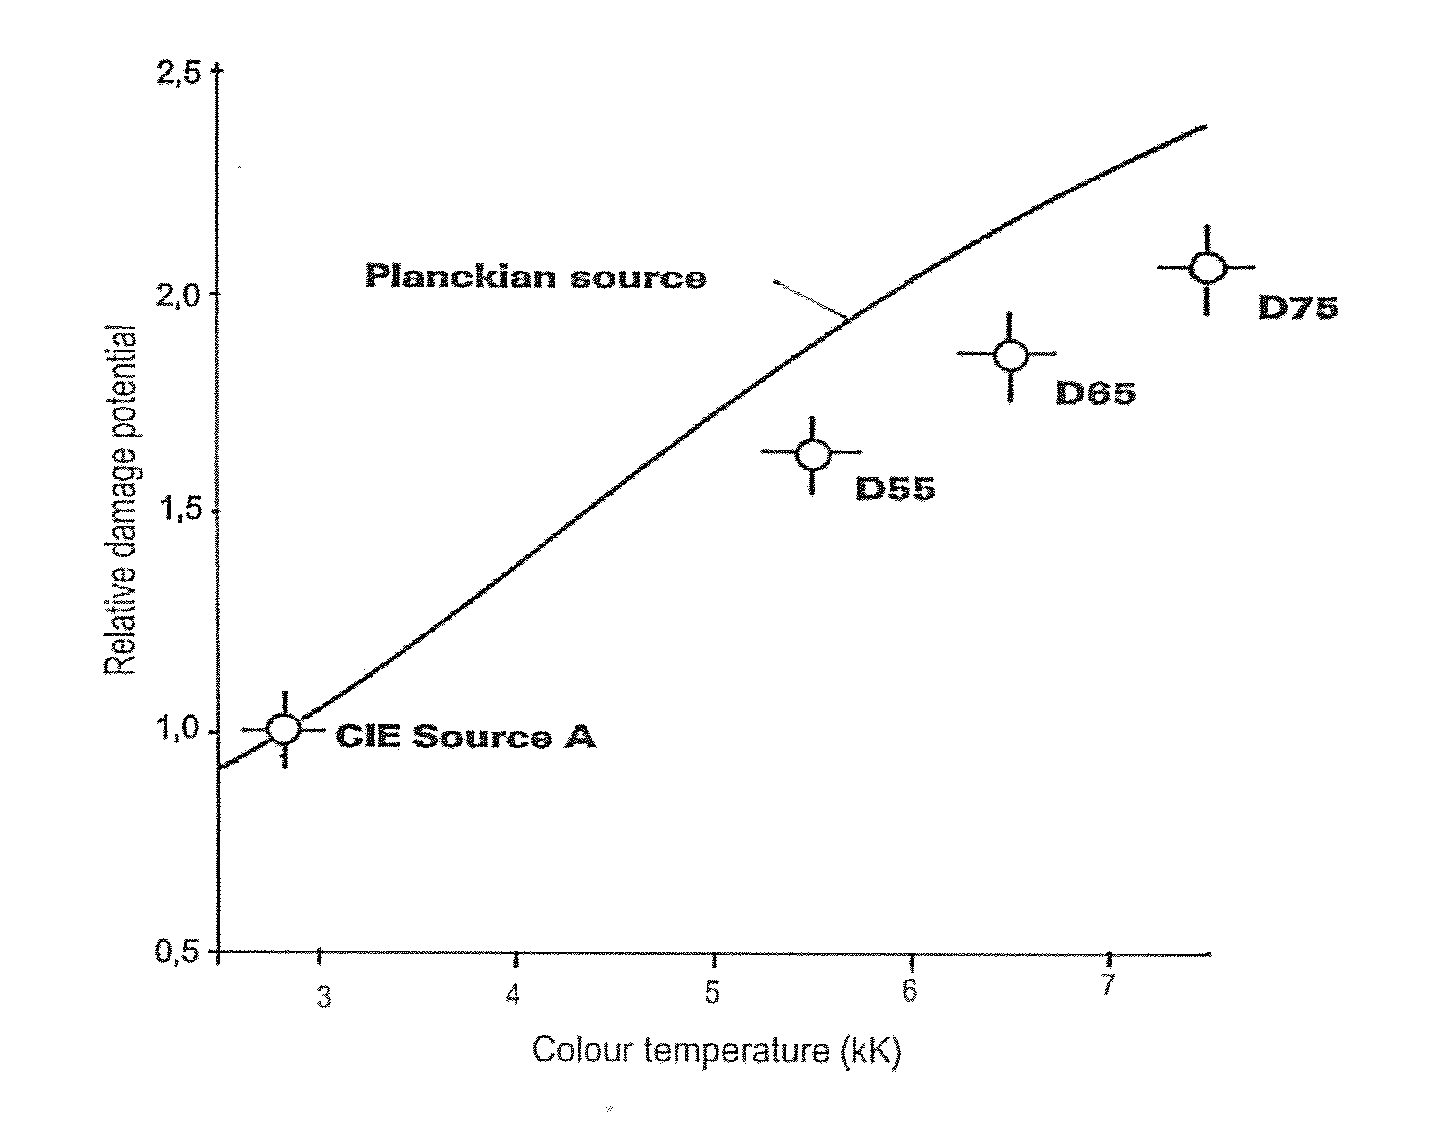
\includegraphics[max width=\textwidth]{figs/LitRev/CIE2004.png} 
\caption{Figure reproduced from CIE 157:2004 \citep[p.16]{cie_cie_2004}, showing the relationship between \gls{CCT} and relative damage potential.}
\label{fig:CIE2004}
\end{figure}

This research relies heavily upon the applicability of damage functions to the specific materials in question. Many (my supervisors) think that damage functions are no good because they're too general, but I would be cautious about throwing the baby out with the bathwater.

\begin{enumerate}
    \item They're the best that we have.
    \item We need something with general applicability anyway - I don't see anyone providing tailored lighting for every object which exists.
    \item The physics checks out.
    \item They're definitely applicable to at least some objects.
\end{enumerate}

To verify the findings of the \gls{CIE}, to extend their findings to \glspl{LED}, and to provide code for others to do similar research or even test their own lights/materials, I wrote some code\footnote{\url{https://github.com/da5nsy/DamageIndex/blob/c7851e27ca1b0915013d8723db04704b49b4085e/CalcDI.m}} which would calculate a \gls{DI}. Then I used that code to compute a new version of the \gls{CIE} plot.

%\afterpage{\clearpage}
%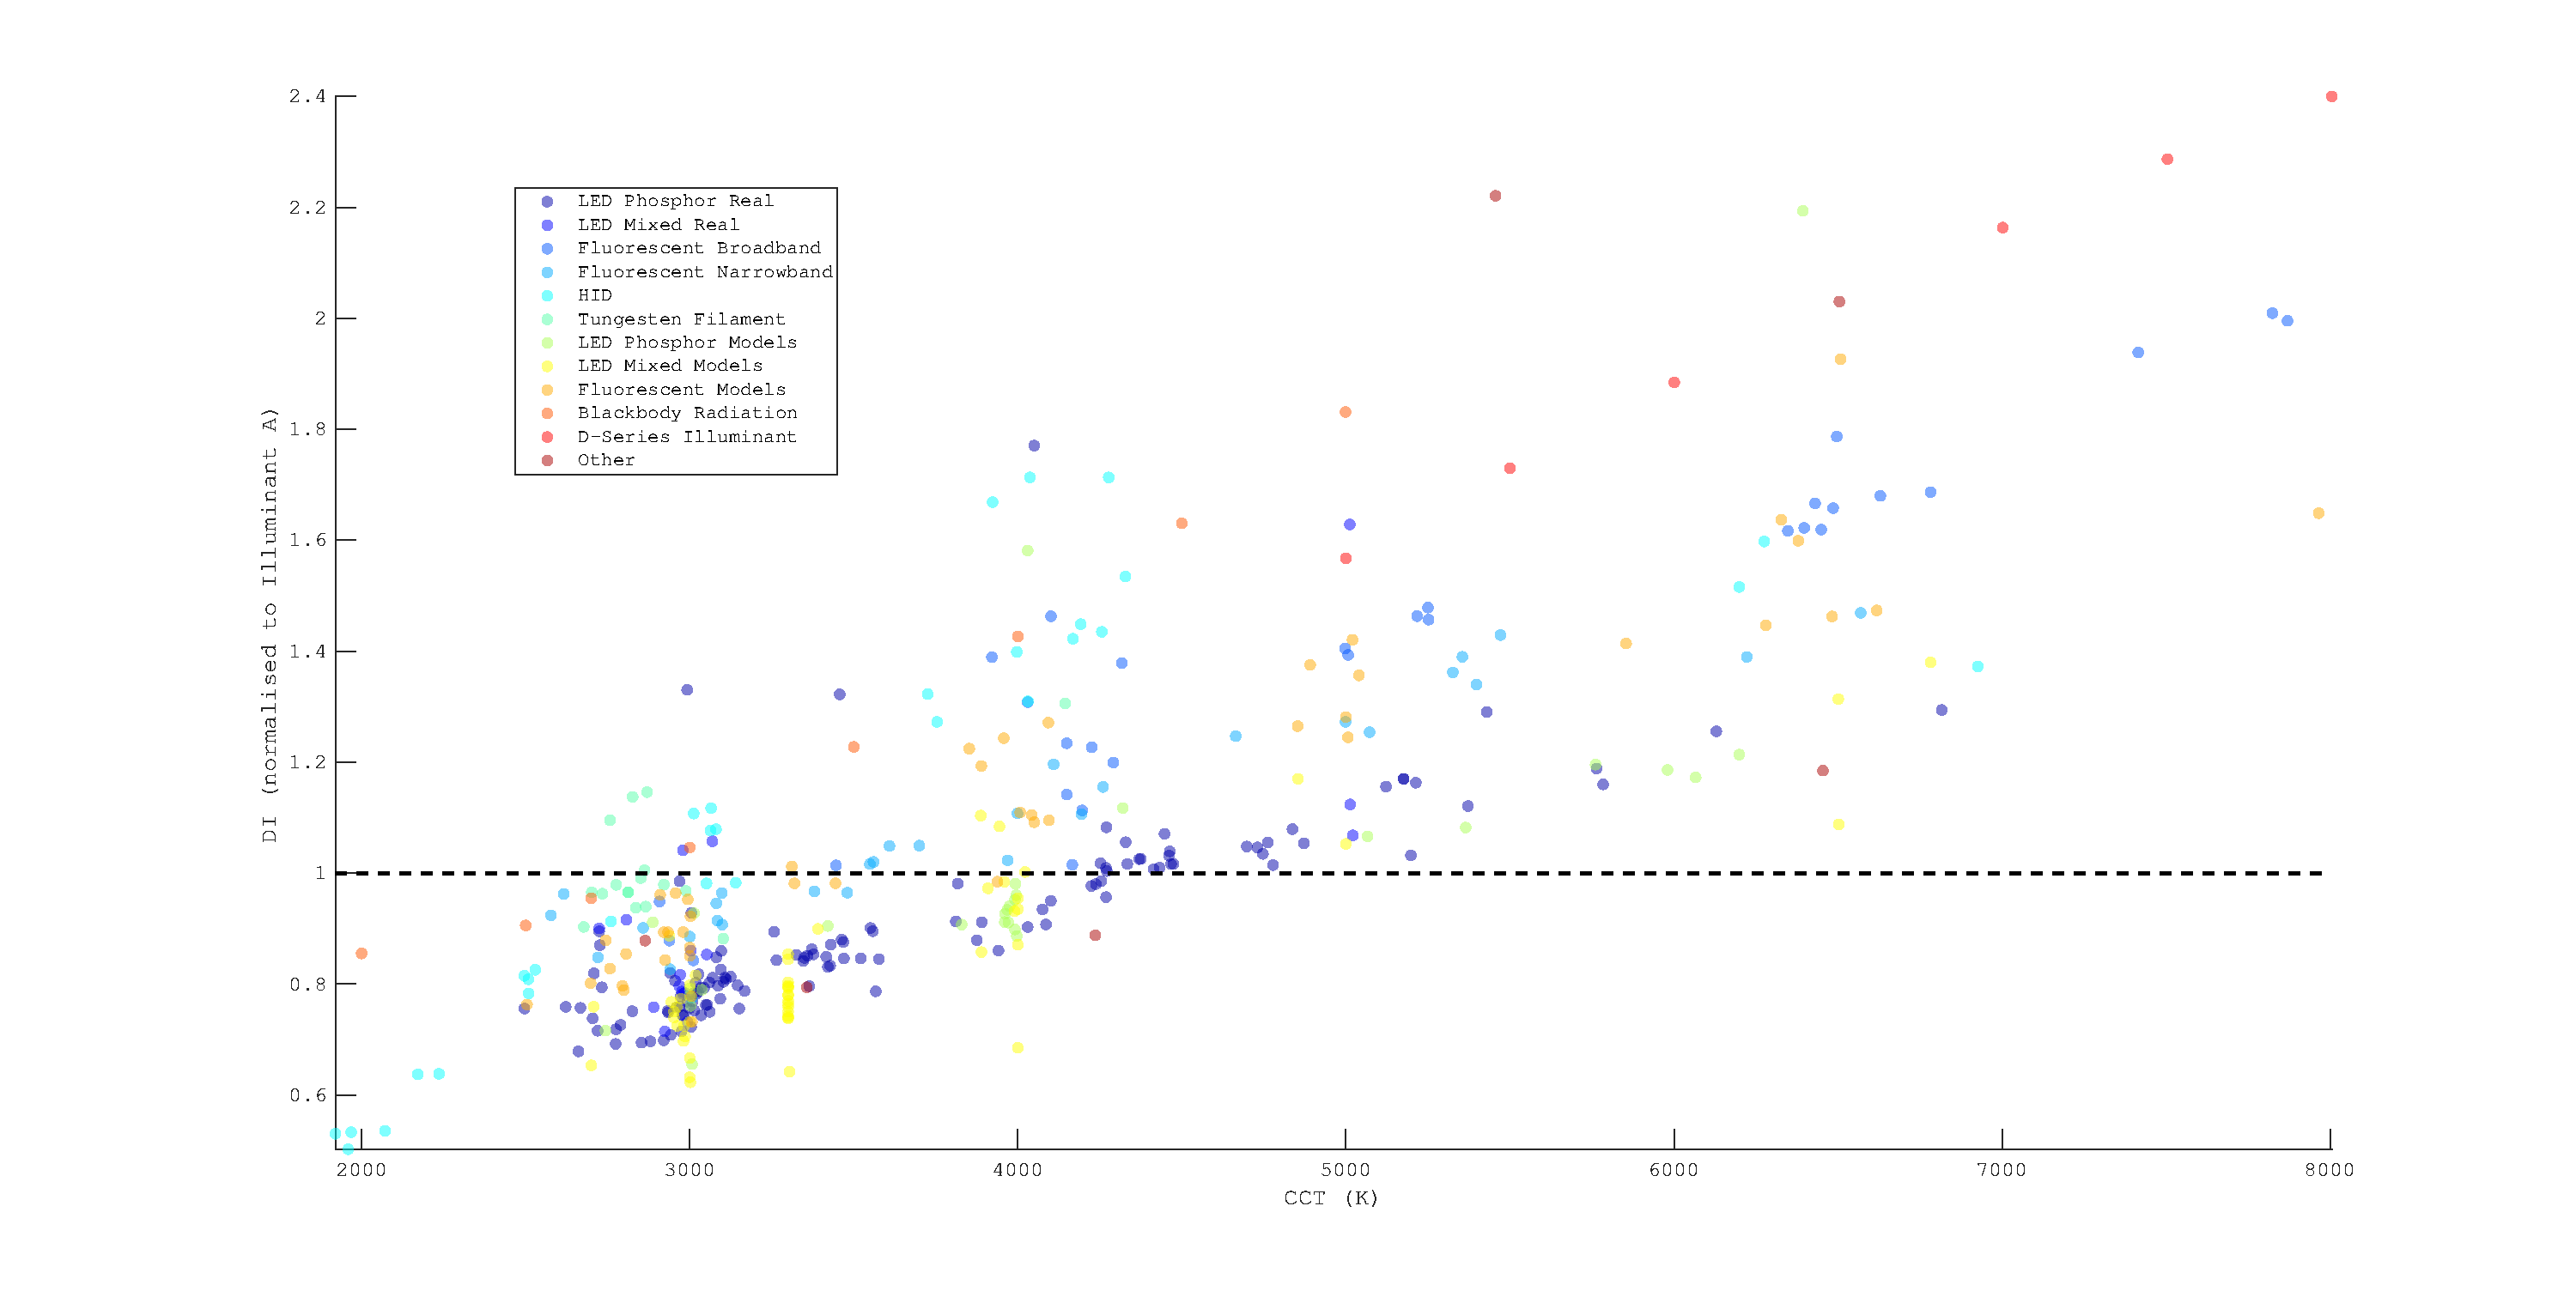
\includepdf[pages=-,rotate=90, offset=75 -75]{figs/LitRev/CCTvsDI.pdf}
% \begin{figure}[t]
%     \caption{The \glspl{CCT} and \glspl{DI} of the \glspl{SPD} used by \citet{houser_review_2013} [provided via personal communication, but now partially available via \gls{PTB} as `spd\_houser'].}
%     \label{fig:CCTvsDI}
% \end{figure} 

\begin{fullpagefigure}
\figpdf[pages=-,rotate=90, offset=75 -75]{figs/LitRev/CCTvsDI.pdf}
\caption{The \glspl{CCT} and \glspl{DI} of the \glspl{SPD} used by \citet{houser_review_2013} [provided via personal communication, but now partially available via \gls{PTB} as `spd\_houser'].}
\label{fig:CCTvsDI}
\end{fullpagefigure}

The results of these computations show a clear relationship between \gls{CCT} and \gls{DI}. Considering that this is not currently taken advantage of in museum lighting, it seems as though there is a great potential for reducing damage whilst maintaining visitor visual satisfaction.

\subsection{Colour Rendering Indices in Museums}

Are fidelity indices suitable for museum use? 
The first chapter of Cuttle's book `Light for Art's Sake: Lighting for Artworks and Museum Displays'19 is titled `A philosophy for the presentation of art'. The choice of title here is apt but may surprise some readers, sounding more whimsical than might be expected of a serious subject attended by scientists and engineers. The reason it is so apt is because lighting is unavoidably a creative intervention (I owe this phrase to Katherine Curran); which is to say that there is no lighting which is truly impartial, and no lighting which is truly correct in the sense of being unequivocally superior to another. All lighting decisions require choices to be made, and whilst these choices can be wrapped up to appear as an optimization problem where proximity to a particular solution is the goal, the problem always rests on the bedrock of a philosophy based decision.

In the above mentioned chapter Cuttle lays out a total of seven distinct philosophical propositions, which he poses for consideration as approaches to museum lighting, some contradictory and some with the potential to overlap:

1.	`To make the artwork appear as it would have appeared to the artist at the time of its creation
2.	To ensure that no damage due to light exposure will occur
3.	To achieve the best possible appearance of the artwork
4.	To provide optimum conditions for viewing art
5.	To impart a sense of having seen `the real thing'
6.	To assist viewers to understand the displayed objects and their reason for being there
7.	For the lighting designer to establish a distinct and recognisable style'19 

These propositions refer to museum lighting holistically, considering all aspects of museum lighting, but can be readily focused on the problem of colour appearance specifically. Before we narrow our gaze however, it is worth briefly considering a wide view of lighting attributes which may aid in the realisation of `good quality' museum lighting. Consider Scott Rosenfeld's list of the five `controllable qualities' in museum lighting; `intensity, movement [temporal artefacts], angle [modelling, avoiding glare and reflections], distribution [ambient lighting vs. spot lighting], color'20.
Whilst Cuttle's propositions make for interesting discussions and enjoyable extended pondering, they are of limited assistance in the practical task of actually specifying lighting. Thankfully, a range of tools exist for the examination of the colour rendering properties of a light source, in the form of indices which aim to numerically describe an illumination's effect on colour appearance of the objects of which it is tasked with illuminating.

Traditionally, colour rendering indices aim to offer a standardized method for calculating the colour differences induced by the substitution of a reference illuminant with a specific test source, and for comparing the relative merit of different test light sources on their ability to induce minimum change. In modern parlance this type of index should be referred to as a colour fidelity index, that is- one which is conceptually concerned with colorimetric reproduction. The term `colour rendering' has come to encompass much more than just fidelity.

Diametrically opposed in some ways to fidelity are the indices which aim to quantify `preference'. In the simplest case, a preference index will aim to provide a value that is predictive of how an observer would rate a light source it against other light sources. 

Within, and on the spectrum between these two groups there exist a range of different indices with subtly different aims and mechanisms for achieving these aims. For a thorough overview, albeit one which omits some more recent developments, see Guo and Houser21.

In practice, both of these philosophical approaches are mandated in current lighting guidance. For the most part, advice for lighting specification6,7 on the subject of colour rendering can be simplified to read `use lamps of above \gls{CRI} 80 (referring tacitly to \gls{CIE} R$_a$) but always test them visually before you buy in bulk'. Whilst this may at first seem like sensible advice, upon further inspection it in fact represents a serious contradiction, unless considered with heavy caveats. The problem rests in the fact that \gls{CIE} R$_a$ is a fidelity index, whereas any visual inspection is likely to be performed by observing the appearance of an object under the test illumination without a reference. Fidelity aims to describe accuracy of reproduction, but this is a quality which is arguably not testable by visual inspection. This contradiction seems to perpetuate unnoticed in museum practice, with lighting specifiers often abstractly declaring to target a faithful/accurate/honest/impartial representation of objects, but practically choosing light sources based on visual inspection where preference is the only criteria. There is of course a range of approaches, ranging from pure reliance on indices to almost entire reliance on visual testing.

In conclusion, no one metric exists that would satisfy the divergent aims and philosophies of museum lighting. Several distinct types of colour rendering index exist, but the existing range fall into the broad categories of `fidelity' or `preference', with the latter being particularly poorly definable due to its variability in different environments, with different user functional requirements and different intrinsic preferences between different observers. Progress could be made by breaking these broad categories into smaller more manageable specific objectives.


%%%% BONUS AREA %%%%%%%%%%


%\subsection{LEDs in museums}

%Theoretically, there exists a division between recommendations which deal with visual appearance and those which deal with physical degradation; the first group supported by the science of human vision, and the second supported by material sciences and chemistry. Whilst it is important to be aware of this distinction, it is normally not possible to consider them entirely separately in practice, as many variables will affect both.


%Extending the question of visibility is the subject of appearance. It is a general expectation that museums represent objects in a truthful and impartial manner, and it seems sensible that decisions concerning the appearance of items in museums should be made with this in mind. Alongside this, many museums treasure items where part of their value is aesthetic2, and it follows therefore that a technique which aids in the beautification of an object might be of interest, and this might be particularly of interest if the object is known to have deteriorated since the time of production.

% \subsection{Lighting at The British Museum}

% Lighting at the British Museum has developed in a somewhat organic manner, from the early days of the museum before the introduction of artificial lighting. This leaves the museum with more than sufficient daylight in most spaces during daylight hours, where the increased modern knowledge regarding the deleterious effect of lighting now means that conservators must find ways in which to limit this natural resource so that objects are not unduly exposed. 

% The gallery lighting is replaced when a gallery is refurbished, and the latest technology is installed when a new gallery is created, where viable in terms of suitability and considering financial limitations. Other than this, lighting technologies tend to not be updated other than to replace individual lamps. This coupled with the grand scope of the museum, which means that it is rare for multiple galleries to be refurbished simultaneously, has led to a vast array of lighting designs and technologies. It in fact appears to represent a rather special example of `museum lighting through the ages', with daylight, tungsten, fluorescent and metal halide lamps all seemingly represented, as well as various illumination geometries reminiscent of the times of their fitting. It should be noted that these assertions are made following empirical observation with spectrophotometers and not from conversations with museum staff, see section 3.3 Collection of \gls{SPD} Data at British Museum.

% There also seems to be a great range of lighting quality within the British Museum, with some spaces feeling bright and others comparatively gloomy. There is a range of colour temperatures and chromaticities of light at the museum, as shown in Figure 1.

% Multiple methods are currently employed to limit the exposure of objects in the museum. \Gls{UV} absorbing film or glazing which incorporates \gls{UV} reduction is used throughout the museum and in certain galleries there are automatic blinds which limit the intrusion of direct sunlight at specific times of the day and year. For particularly sensitive objects, rooms are lit artificially at very low levels, and some objects are selectively lit in order to further limit their accumulative exposure.

% 